%!TEX root = thesis.tex
\todo{flavour billeder til afsnittet}
\section{A historical overview}
We will first give a brief overview of the evolution of computer interfaces.
These is of cause many ways to look at the evolution of the computer and the computer interface. 

Alongside these shifts in computer generations there has also been quite a development, both in the way we can interact and manipulate the computer, but also in the computer's knowledge about its user.
In traditional computer systems there have always been a strong separation between the user and the machine, the physical world and the digital world.
In this section we will take a look at how the relation between physical and digital has evolved though time.

\subsection{Computer interaction}
\todo{afsnit skal have nogle referencer}
Looking back in time to the early digital computers of the 1940s and 1950s these systems were interacted with though punch cards.
Punch cards represents digital information by the presence or absence of holes on the card, based on a predefined pattern which the computer could then read.
The user would use a machine to punch holes in the cards with either programming commands that could be run on the computer or as an analogue data storage that could later be read by the computer.
From a human perspective the punch cards is an abstract non-readable input form that very much works on the premises of the computer.
An interesting aspect of the punch card technology is that the user interacts with the digital layer of the computer though a physical token that represents the digital information (the card itself).
This approach to interaction gets reinvented as a novel interaction form much later, in the form of Tangible User Interfaces (TUIs), which will be described later in this section.
(It is of cause a stretch to classify punch cards as a TUI as it lacks many of the defining properties.) 

A few decades later the command-line interface begins to gain traction with a text-based input and output system that are readable by humans.
The user issues commands to the computer by typing lines of text commands and gets a visual response on the monitor.
The challenge here is it strictly command driven and that the user has to know which commands the computer provides to be able to interact with it, but once you master the commands it can provide a fast and efficient interaction.
For this reason it is, still today, mostly used by expert users, as there is a lack of physical and/or visual metaphors to link the command language to the real world to make it intuitive.  
The physical and digital world is still very much separated although the language of interaction, bridging the two world, does incorporate some human aspects by being directly readable, but not necessarily easily understood.

With the emergence of the computer mice and more powerful computers, the Graphical User Interface(GUI) became, and still is, the most popular method of interacting with the computer.
GUIs make use of visual metaphors inspired by the real world to guide the users actions and understanding of the system.
The most obvious being the desktop metaphor that links the office space to the computer with digital folders, documents, trash bins and so on, simulating a physical desktop on the monitor.
Using metaphors in this way can ease the user's annexation into the digital world as they, if done properly, creates logical links between knows physical actions and potential digital actions.

Virtual Reality (VR) systems puts even more of the physical world in to the digital environment.
Instead of using metaphors from the real world the goal here is to create a virtual representation of a physical world, giving the user a simulated feeling of physical presence in the digital environment.
This approach very clearly separates the digital and physical layer as the digital environment only simulates a physical space without affecting it or being affected by it.

As an opposite to VR systems attempt to create digital representations of the real world, we find TUIs.
TUI systems attempts to create physical representations of the digital state of the computer, embedding a digital layer into physical objects and environments.
The term was first coined by \cite{ishii1997tangible}, building on Weiser's vision of the ubiquitous and invisible computer.
Ishii and Ullmer states two goals for TUIs:
\begin{itemize}
		\item{allowing users to ``grasp and manipulate'' foreground bits by coupling bits with physical objects, and}
		\item{enabling users to be aware of background bits at the periphery using ambient media in an augmented space}
\end{itemize}
By embodying digital information into tangible objects, TUI systems takes advantage of humans ability to sense, interact and manipulate the physical world. 

\todo{videre herfra}

\subsection{Computer generations}
Another interesting aspect of the evolution of computers to look at the changes to the user's relation to the computer.
A simple way to look at the at this, on a broad scale, is to divide the changes into generations based on the relation between the user and the computer system.
Abowd \citep{abowd2012next} mentions three overall generation.
1\textsuperscript{st} generation being terminal based computing where multiple users share the same computer in a many-to-one relationship.
In the 2\textsuperscript{nd} generation the personal computing revolution happens and it becomes possible to have a one-to-one relationship between the computer and the user.
The 3\textsuperscript{rd} generation being ubiquitous computing, the concept defined by Mark Weiser in his key article \cite{weiser1991computer}.
Here a one-to-many relationship becomes reality as a single person now interact with multiple computers. Computers become an integrated part of every day objects and every day life. 
As Abowd correctly notes, Weiser's vision has to some extend become reality. 
Computers are part of the environment and have indeed been \textit{woven} into the fabric of everyday life in many ways. \todo{giv nogle simple eksempler}  

\section{A possible future for user interfaces}
If we are beginning to pass the 3\textsuperscript{rd}, Abowd asks \textit{so, what's next?}.
This is of cause a complex and difficult question to answer.
Abowd suggests a future where the human-computer experience is more conjoined than ever, blurring the boundaries between them.
\begin{quote}
\emph{[\ldots] our own physical being and our sense of identity is no longer easily distinguished from elements of computing.}
\end{quote}
Abowd also touches on a topic that has been dominant in the last few years, namely cloud computing.
Broadly seen cloud computing refers to services and applications that are made available over a network \todo{wiki ref?}.
This could be data storage, computing power, back-up services or applications which makes traditional desktop applications available through the Internet.
Abowd suggests that future devices will be able to adapt to whoever is currently using it, as all relevant information will available be in from the cloud.
Following this, devices and their services no longer have to be closely ties together, leading the way for genetic multi purpose devices that delivers services from the cloud.

\cite{ishii2012radical} presents an alternative vision for the future.
They presents the vision as \textit{Radical Atoms}, a vision for the future of \textit{human-material interaction} or \textit{material user interface}. 

\todo{noget med shape change - ledende op til SC afsnit og vores protype og ide om ad hoc interfaces}
\todo{3.wave HCI bødker}

\section{Shape Changing Interfaces}
\subsection{Introduction}
Shape-changing interfaces (SCIs) are a relative new subject in the area of human-computer interaction.
In previous work it has been discussed under various different terms such as Kinetic Interaction, Organic User Interfaces, Actuated Interfaces, to name a few stated by \cite{rasmussen2012shape}.

\subsection{A vocabulary of shape-change}
In this chapter we will expand our vocabulary regarding SCIs based on \cite{coelho2011shape} and \cite{rasmussen2012shape}.
They both provide contributions as to how we can talk about SCIs, how we can group and identify different types of change of shape, how we can identify and describe shape transformations, and most importantly, how and to which purpose we can interact with SCIs.
We will use this vocabulary onwards in our thesis to discuss SCIs, both ours and others.   
Rasmussen defines shape-changing interfaces as
\begin{quotation}
\emph{A shape-changing interface uses physical change of shape as input or output.}
\end{quotation}
and further
\begin{quotation}
\emph{[\ldots] the self-actuation must be controllable so that the object can return to its initial state and repeat the shape change.}
\end{quotation}

\cite{coelho2011shape} presents a grouping which distinguish three types of change of shape: \emph{topological, textural and permeable} transformations.
Topological transformations here being those transformations which adhere to topological equivalence, permeable those which do not and textural transformation stands as a category for it. Topologically equivalence here means that a form can transform in to another form by a continuously homeomorphic transformation - that is without cutting or gluing either form. This can be exemplified by the pliable donut that transforms into a coffee mug without breaking homeomorphism as seen in figure~\ref{pliable-mug} \todo{lav egen figur?} 

\begin{figure}[hb]
	\centering
  		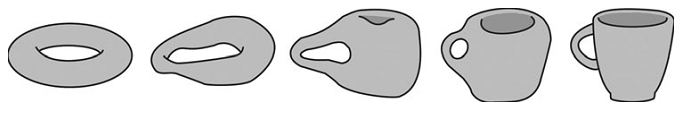
\includegraphics[width=4in]{figures/pliable-donut}
	\caption[The pliable donut momeomorphic transformation \cite{coelho2011shape}]
   {The pliable donut momeomorphic transformation \cite{coelho2011shape}}
   \label{pliable-mug}
\end{figure}   
 
\cite{rasmussen2012shape} suggests a grouping more detailed grouping of shape-changing interfaces by identifying eight types of change of shape, namely: \textit{orientation, form, volume, texture, viscosity, spatiality, adding/subtracting and permeability}.
These eight fit into two groups where the first six are topologically equivalent and the last two are not. This is in line with what \cite{coelho2011shape}, though texture standing has been moved into the topologically equivalent group. Overall it expands on \cite{coelho2011shape}s work and enables us to identify and discuss form changes in more detailed terms.
The grouping is visualized in figure~\ref{types-of-change}, illustrating the different types of change.

\begin{figure}[hb]
	\centering
  		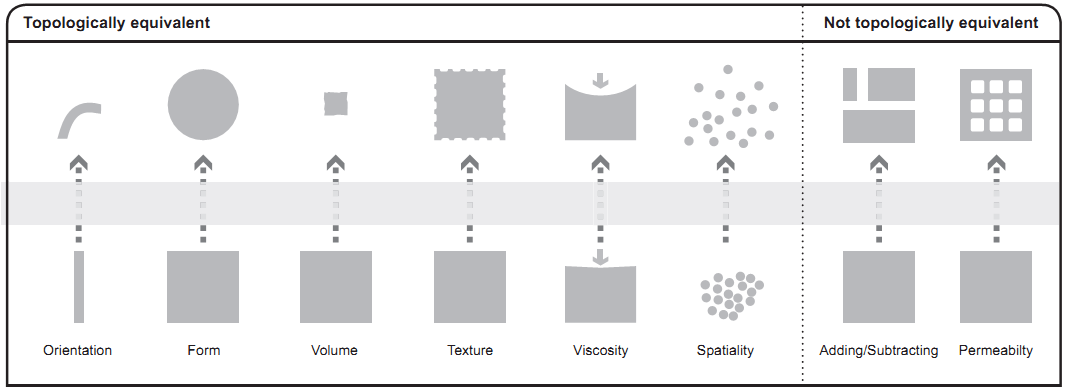
\includegraphics[width=4in]{figures/types-of-change}
	\caption[Types of shape-change as visualised by \cite{rasmussen2012shape}]
   {Types of shape-change as visualised by \cite{rasmussen2012shape}}
   \label{types-of-change}
\end{figure}

There might be some debatable cases in this grouping, e.g. they define textural change as
\begin{quotation}
small changes on the surface of the shape that add visual and tactile properties without affecting the overall form
\end{quotation} 
so if the overall form is not changed it might not make sense to classify it as a homomorphic transformation, which might also be the reason why \cite{coelho2011shape} chose to separate it as a case for itself.
Also if we look at the case of spatiality changes where a collection of elements form a single object, it is possible to think of examples where non-homeomorphic transformations occurs if, for example, the collection of elements split in the middle forming two objects and then merge back together.
This would still count as a shape-changing interface as described in the definition but would not adhere to topological equivalence.   

The transformation in itself is interesting as well and \cite{rasmussen2012shape} reveals different types of transformation.  They describe the transformation as the \textit{phase between endpoints}, meaning the phase between the form's origin and its morphed state.
They distinguish between kinetic parameters and expressive parameters, where
the kinetic parameters describe the physical movements of the transformation and the expressive parameters relates to how the kinetic movements are perceived and understood.
This is a very interesting and important aspect of SCIs since it, together with the theory of affordances, provides the basis for understanding the interface and its functions, which at the same time is one of the key challenges of SCIs.
Since SCIs are inherently non-static objects we might not be able to rely on the form alone to communicate the intent and functions of the object, so there might have to be some interaction clues elsewhere, for example in the transformation itself. This will be discussed in more detail in chapter \todo{ref somewhere}  

A key aspect of SCIs, and any user interface in general, is the interaction - be it direct physical interaction, implicit visual interaction, or something in between. 
\cite{rasmussen2012shape} distinguish between \textit{no interaction}, where there is only shape-changing output; \textit{indirect interaction}, still only with shape-changing output but based on implicit user input; \textit{direct interaction}, where the user deforms the object in some way as user input and a shape-change output occurs, either in the object itself or in a remote object.
Two approaches to direct interaction are identified, \textit{action and reaction} where the object reacts directly to the action in a synchronized process and \textit{input and output} where the object is acting asynchronously and not necessarily directly related to the input.    
Our focus will be on objects with direct interaction and mainly those with input and output merged into the same object, as we here see the best possibilities for creating interfaces \todo{et eller andet}
 
\hl{Our own exploratory work will focus only on topological transformations, excluding spatiality, since our choice of technology hinders this type of change.} This will be further described in section \todo{ref til proto 0}  

